\clearpage\appendices
\section{Árvores temporais completas}
\noindent\textbf{Leitura.} A identifica tarefa abstrata, U interna do usuário, I interativa e S do sistema. $\gg$ impõe sequência; $[\,]\gg$ transmite o resultado ao sucessor; $[\,]$ entre tarefas oferece escolha; $|||$ permite intercalação; $|=|$ permite qualquer ordem sem intercalação. Colchetes em torno de uma tarefa indicam opcionalidade e o asterisco indica repetição. Os números recuperam as operações da HTA. Ao ler um cartão de V1, etiquetas $|=|$ preços permite conferir integralmente um ou outro primeiro. O rótulo da apresentação não presume leitura mental.
\par\smallskip Para cada raiz $T$, aplica-se $(T\,|>\,\text{consultar ajuda})\,[>\,(\text{desistir}\,[\,]\,\text{atingir limite}\,[\,]\,\text{falhar})$. A consulta suspende e retoma: solicitar ajuda (I) $\gg$ apresentar dica (S) $\gg$ [escolher camada (I) $\gg$ apresentar conteúdo (S)]* $\gg$ fechar (I) $\gg$ restaurar origem (S). A desativação termina por desistência (I), limite (S) ou falha técnica (S). O suporte fica fora dos métodos especialistas.
\par\smallskip\noindent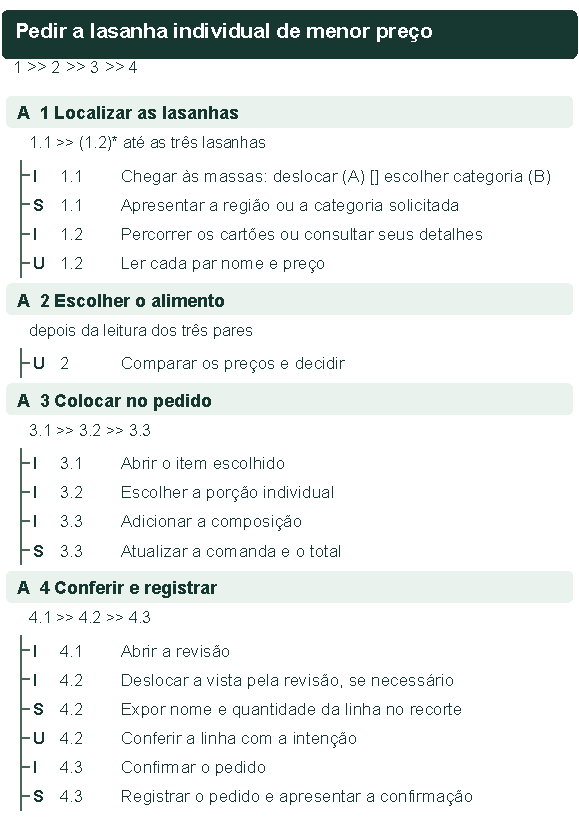
\includegraphics[width=\columnwidth]{../design/figures/CTT-C1.pdf}
\par\smallskip\noindent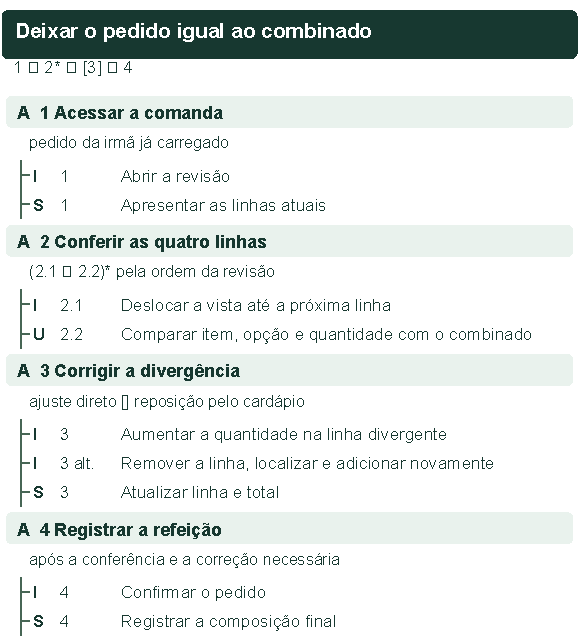
\includegraphics[width=\columnwidth]{../design/figures/CTT-C2.pdf}
\par\smallskip\noindent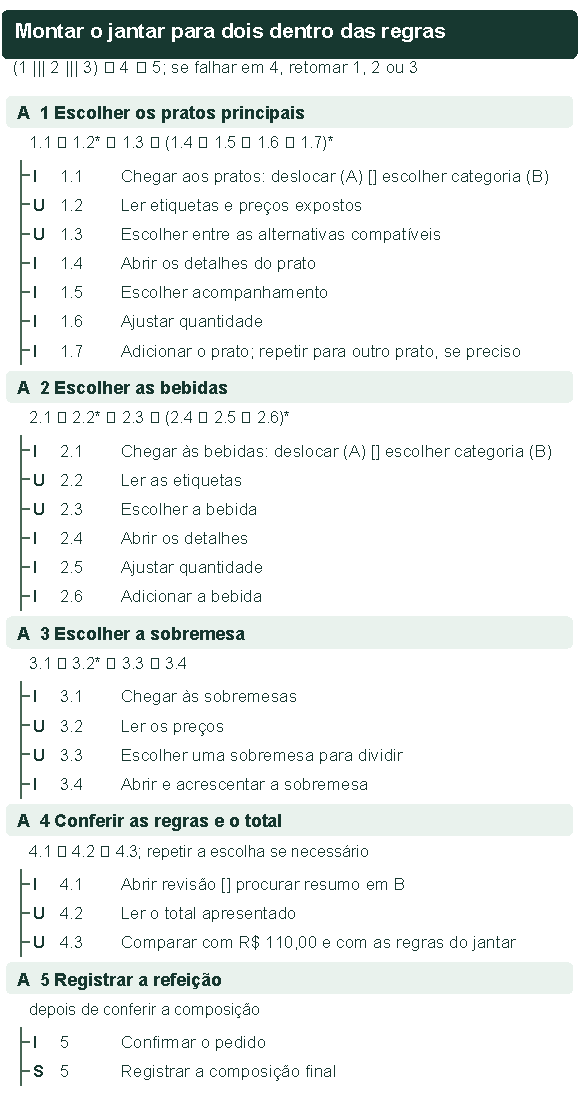
\includegraphics[width=\columnwidth]{../design/figures/CTT-V1.pdf}
\par\smallskip\noindent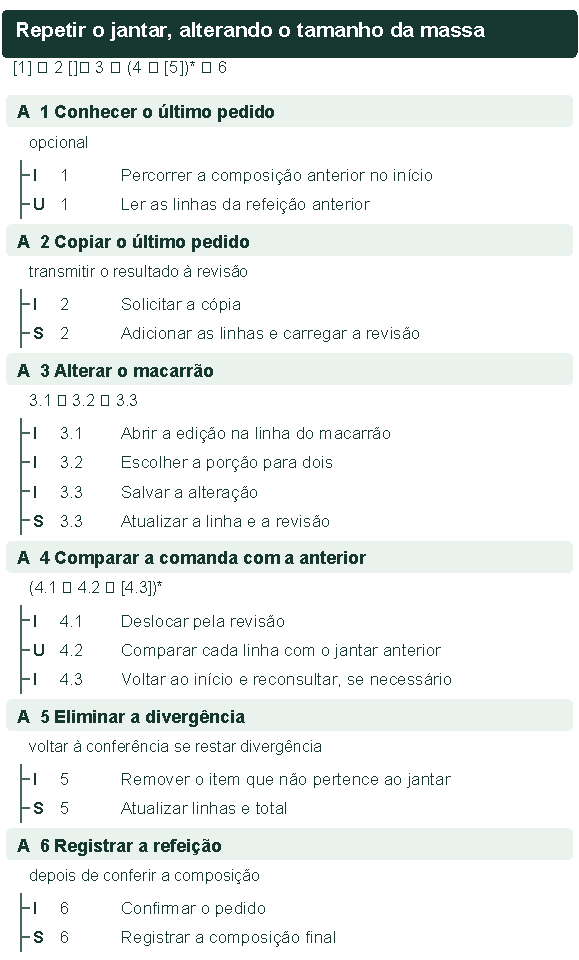
\includegraphics[width=\columnwidth]{../design/figures/CTT-V2.pdf}
\section{Diálogo e esboços do protótipo}
\noindent\textbf{MoLIC.} As cenas delimitam assuntos, P identifica processos e as guardas limitam atos de fala. O subdiálogo S5 preserva a cena de origem. Ajustar a vista conserva o assunto corrente. A desistência encerra a sessão em curso.
\par\smallskip\noindent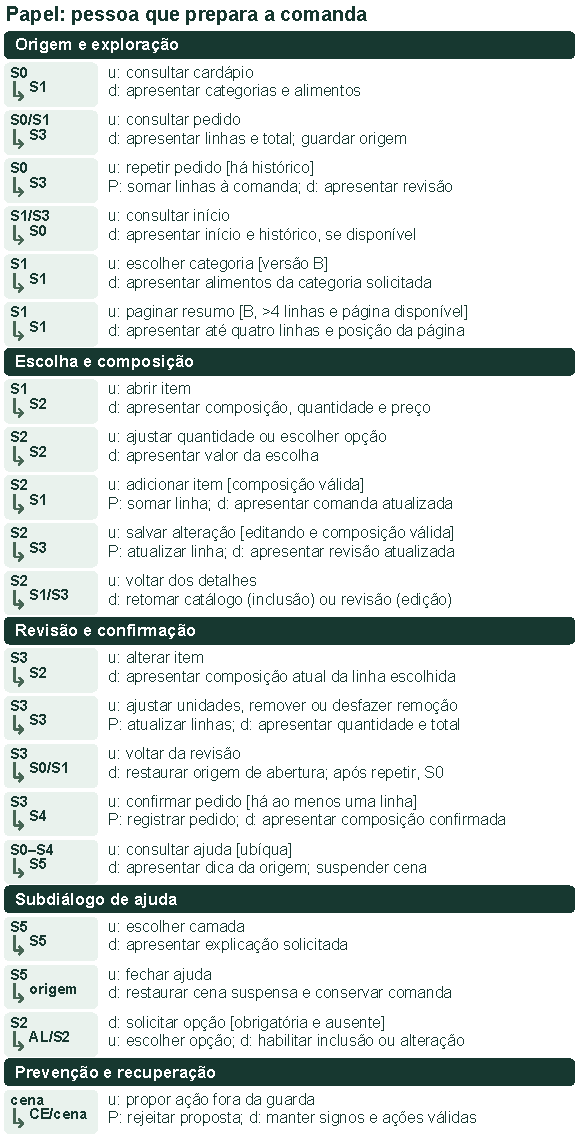
\includegraphics[width=\columnwidth]{../design/figures/MoLIC.pdf}
\par\smallskip\noindent\textbf{Esboços.} Cada quadro mostra a hierarquia dos signos e o ponto de acesso ao suporte. A linha de um pedido concreto inclui opção, quantidade e valor. O painel de pesquisa fica fora da projeção do agente.
\par\smallskip\noindent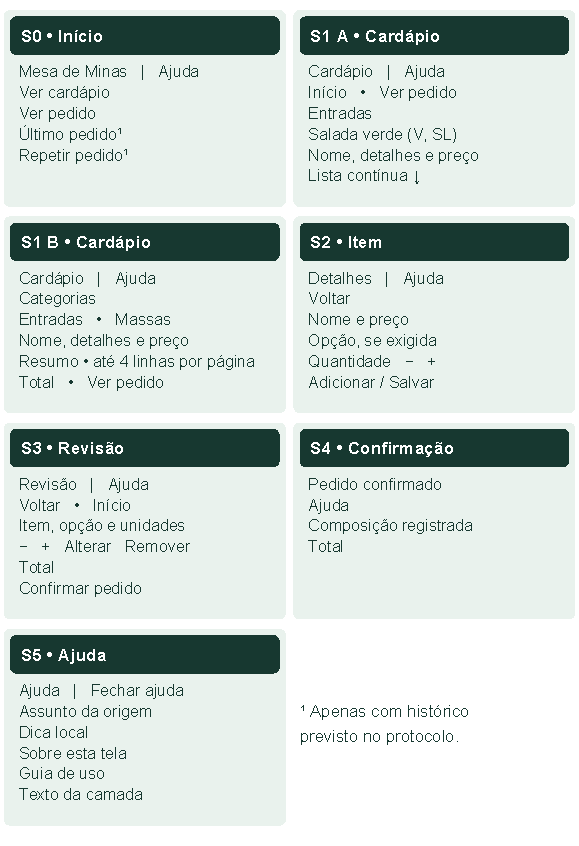
\includegraphics[width=\columnwidth]{../design/figures/Wireframes.pdf}
\section{Esquema conceitual de signos}
\noindent O esquema descreve cada signo usado nas tarefas pelo conteúdo e pela expressão. Não é o modelo de dados. A coluna \emph{Na observação do agente} aplica a equivalência de canal: \emph{trecho} é o texto geométrica e tipograficamente legível no recorte; abaixo do limiar de legibilidade restam o tipo do elemento e sua posição. Nenhum identificador interno, estado lógico de desabilitação ou elemento fora do recorte entra na observação. A coluna \emph{Evento} liga o signo ao registro do pesquisador. Os signos de aplicação recebem explicação completa nas três camadas da ajuda.
\newcommand{\SGhead}{\hline \textbf{Signo (entidade.atributo)} & \textbf{Origem} & \textbf{Conteúdo (tipo, restrições, default)} & \textbf{Expressão (widget)} & \textbf{Tipo} & \textbf{Na observação do agente} & \textbf{Evento}\\ \hline}
\begin{table*}[!t]
\caption{Esquema conceitual de signos estendido (parte 1: cardápio, item e navegação)}
\label{tab:signos1}
\centering\scriptsize\setlength{\tabcolsep}{3pt}\renewcommand{\arraystretch}{1.08}
\begin{tabularx}{\textwidth}{@{}>{\raggedright\arraybackslash}p{.135\textwidth}>{\raggedright\arraybackslash}p{.085\textwidth}>{\raggedright\arraybackslash}X>{\raggedright\arraybackslash}p{.15\textwidth}>{\raggedright\arraybackslash}p{.085\textwidth}>{\raggedright\arraybackslash}p{.165\textwidth}>{\raggedright\arraybackslash}p{.13\textwidth}@{}}
\SGhead
Restaurante.nome & domínio & texto; denominação do restaurante ou da lanchonete de treino & cabeçalho & estático & trecho legível & \UXev{elemento_visto}\\
Tela.assunto & aplicação & enumerado S0--S5; cena corrente & título da tela & estático & trecho do título & \UXev{tela_alterada}\\
Início.histórico & domínio & lista das linhas do último pedido, quando prevista na tarefa & relação de itens & estático & trechos de linhas & \UXev{elemento_visto}\\
Pedido.repetição & aplicação & ação; acrescenta as linhas históricas às atuais & botão Repetir pedido & estático & alvo visível & \UXev{item_adicionado}\\
Navegação.destino & convencional & enumerado: início, cardápio ou revisão & controles de navegação & estático & alvo visível & \UXev{tela_alterada}\\
Navegação.retorno & convencional & ação; abandona edição pendente & botão Voltar & estático & gesto ou alvo corrente & \UXev{tela_alterada}\\
Categoria.nome & domínio & texto; cinco categorias na ordem herdada & seção (A) ou aba (B) & estático & trecho & \UXev{elemento_visto}\\
Categoria.ativa & aplicação & enumerado; default: entradas (somente B) & realce da aba & dinâmico & pistas visíveis e itens expostos & \UXev{tela_alterada}\\
Item.nome & domínio & texto do catálogo; 30 itens & cabeçalho do cartão & estático & trecho, sem completar vizinhos & \UXev{elemento_visto}\\
Item.descrição & domínio & texto; ingredientes ou preparo & texto do cartão & estático & trecho & \UXev{elemento_visto}\\
Item.etiquetas & transformado & conjunto de \{V, SL, SA\}, possivelmente vazio & marcas junto ao item & metalinguístico & somente o próprio trecho & \UXev{elemento_visto}\\
Item.preço & domínio & centavos inteiros positivos; dois preços para massas & valor em reais & estático & trecho monetário & \UXev{elemento_visto}\\
Item.detalhes & aplicação & ação; abre a composição do item tocado & cartão tocável & estático & alvo visível, sem identificador interno & \UXev{tela_alterada}\\
Item.opção & domínio & tamanho ou acompanhamento obrigatório; default: nenhuma escolha & grupo de opções & dinâmico & textos expostos & \UXev{opcao_selecionada}\\
Opção.exigência & aplicação & condição para incluir o item & aviso escrito & metalinguístico & trecho do aviso, sem marca lógica de desabilitação & \UXev{elemento_visto}\\
Item.quantidade & domínio & inteiro $\geq 1$ & número e controles $+/-$ & dinâmico & número ou sinal visível & \UXev{acao_executada}\\
Item.inclusão & aplicação & ação; efetiva uma nova linha & botão Adicionar & dinâmico & alvo visível admissível & \UXev{item_adicionado}\\ \hline
\end{tabularx}
\end{table*}
\begin{table*}[!t]
\caption{Esquema conceitual de signos estendido (parte 2: pedido, ajuda, vista e protocolo)}
\label{tab:signos2}
\centering\scriptsize\setlength{\tabcolsep}{3pt}\renewcommand{\arraystretch}{1.08}
\begin{tabularx}{\textwidth}{@{}>{\raggedright\arraybackslash}p{.135\textwidth}>{\raggedright\arraybackslash}p{.085\textwidth}>{\raggedright\arraybackslash}X>{\raggedright\arraybackslash}p{.15\textwidth}>{\raggedright\arraybackslash}p{.085\textwidth}>{\raggedright\arraybackslash}p{.165\textwidth}>{\raggedright\arraybackslash}p{.13\textwidth}@{}}
\SGhead
Pedido.resumo & transformado & composição e total; somente em B & rodapé fixo & dinâmico & apenas a interseção efetiva com o recorte & \UXev{elemento_visto}\\
Resumo.página & aplicação & até quatro linhas por página; Anterior/Próxima quando há página nessa direção & paginação do rodapé (B) & dinâmico & alvos e linhas expostos & \UXev{acao_executada}\\
Linha.composição & transformado & nome, opção, unidades e subtotal & linha da revisão & dinâmico & fragmentos expostos & \UXev{elemento_visto}\\
Linha.unidades & transformado & inteiro positivo da linha existente & controles $+/-$ & dinâmico & controle visível & \UXev{item_alterado}\\
Linha.edição & aplicação & ação; reabre os detalhes da linha e aplica a mudança & botões Alterar e Salvar alteração & dinâmico & alvo do recorte & \UXev{item_alterado}\\
Linha.remoção & aplicação & ação; exclui a linha escolhida & botão Remover & dinâmico & alvo visível & \UXev{item_removido}\\
Linha.reposição & aplicação & ação; recupera a última remoção disponível & botão Desfazer remoção & dinâmico & alvo visível & \UXev{item_adicionado}\\
Pedido.total & transformado & soma dos subtotais, em reais & valor total & dinâmico & trecho & \UXev{elemento_visto}\\
Pedido.vazio & aplicação & ausência de linhas & mensagem & dinâmico & trecho & \UXev{elemento_visto}\\
Pedido.registro & aplicação & ação; exige comanda não vazia & botão Confirmar pedido, depois mensagem e linhas & dinâmico & alvo e resposta no recorte & \UXev{pedido_confirmado}\\
Ajuda.acesso & aplicação & ação; solicita explicação da cena & botão Ajuda ou F1 & estático & alvo visível ou acesso ubíquo previsto & \UXev{ajuda_aberta}\\
Ajuda.camada & aplicação & enumerado: dica local, sobre esta tela, guia de uso & três escolhas & dinâmico & opções da ajuda aberta & \UXev{ajuda_aberta}\\
Ajuda.tópico & aplicação & texto do assunto da cena de origem na camada escolhida & título e texto & metalinguístico & trecho, somente após a abertura & \UXev{observacao}\\
Ajuda.retorno & convencional & ação; retoma a cena de origem & botão Fechar ajuda ou Esc & estático & alvo visível & \UXev{ajuda_fechada}\\
Vista.escala e posição & convencional & janela de $360/z$ por $800/z$ px CSS e posição & gestos de ampliar, reduzir e deslocar & dinâmico & recorte e gestos permitidos & \UXev{zoom_alterado}, \UXev{vista_deslocada}\\
Protocolo.instrução & aplicação & enunciado literal e estável da tarefa & texto do protocolo & metalinguístico & texto literal & \UXev{tarefa_iniciada}\\
Protocolo.saída & convencional & ação; interromper por iniciativa própria & gesto Desistir & dinâmico & gesto de protocolo & \UXev{desistencia}\\ \hline
\end{tabularx}
\end{table*}

\section{Texto das três camadas de ajuda}
\par\smallskip\noindent\textbf{S0}
\par\noindent\emph{Dica local.} Consulte o cardápio para começar. Se houver um último pedido, você pode consultá-lo aqui.
\par\noindent\emph{Sobre esta tela.} O último pedido mostra a composição registrada anteriormente. Repetir pedido acrescenta esses itens ao pedido em andamento. Confira também os itens que já estavam nele.
\par\noindent\emph{Guia de uso.} Para começar de novo pelo cardápio, escolha Ver cardápio. Para usar uma composição anterior, escolha Repetir pedido, se disponível. Na revisão, confira as opções e as quantidades. O pedido é registrado quando você o confirma.
\par\smallskip\noindent\textbf{S1}
\par\noindent\emph{Dica local.} Cada item tem nome, descrição e preço. Consulte o item para conhecer as opções disponíveis.
\par\noindent\emph{Sobre esta tela.} Na lista contínua, os itens aparecem por categoria. Na versão com categorias, escolha o nome da categoria para ver seus itens. Ver pedido abre a revisão. O resumo no rodapé, quando presente, acompanha o pedido em andamento.
\par\noindent\emph{Guia de uso.} As etiquetas pertencem ao item junto do qual aparecem. (V) significa vegetariano, (SL) significa sem lactose e (SA) significa sem açúcar ou sem açúcar adicionado. Consulte os detalhes, escolha as opções desejadas e acrescente o item. Você pode rever o pedido antes de confirmar.
\par\smallskip\noindent\textbf{S2}
\par\noindent\emph{Dica local.} Confira o nome e o preço do item. Quando houver uma opção obrigatória, escolha-a antes de acrescentar ou salvar.
\par\noindent\emph{Sobre esta tela.} O acompanhamento compõe o prato principal. O tamanho define a porção de massa. A quantidade indica quantas unidades da combinação serão pedidas. Aumente ou diminua a quantidade pelos controles junto ao número.
\par\noindent\emph{Guia de uso.} Ao incluir um item, escolha a opção, ajuste a quantidade e use Adicionar. Ao modificar uma linha existente, use Salvar alteração. Para sair dos detalhes antes de aplicar a escolha, use Voltar.
\par\smallskip\noindent\textbf{S3}
\par\noindent\emph{Dica local.} Confira cada linha, suas opções e quantidades. O total reúne todas as linhas do pedido.
\par\noindent\emph{Sobre esta tela.} Use os controles junto à quantidade para ajustá-la. Alterar permite rever as opções da linha. Remover retira a linha do pedido. Confira o nome junto dos controles antes de fazer uma alteração.
\par\noindent\emph{Guia de uso.} Percorra o pedido e confira as linhas com o que deseja receber. Para recuperar uma linha, use Desfazer remoção enquanto essa opção estiver disponível. Você também pode voltar ao cardápio e acrescentar o item novamente. Ao terminar a conferência, use Confirmar pedido.
\par\smallskip\noindent\textbf{S4}
\par\noindent\emph{Dica local.} A confirmação indica que o pedido foi registrado.
\par\noindent\emph{Sobre esta tela.} O registro conclui a composição do pedido neste restaurante fictício. A confirmação informa que a operação terminou.
\par\noindent\emph{Guia de uso.} Consulte a mensagem de confirmação para reconhecer o fim do pedido. Esta demonstração não processa pagamentos nem envia pedidos a restaurantes.

\section{Rastreabilidade e registro de decisões}
\begin{uxtable}{Perfil e tarefa}{Mecanismo, signo, registro e estatuto}
\UXrow{M1, C1\,1 e 4}{Ampliação $\rightarrow$ recorte e legibilidade $\rightarrow$ nome/preço $\rightarrow$ deslocamentos por item ($D$). E para amplitude observada, HO para limiar e geometria.}
\UXrow{M2, C1\,2}{Contexto ausente $\rightarrow$ memória FIFO de fragmentos $\rightarrow$ comparação de preços $\rightarrow$ revisita ($V$). E indireta para perda do contexto, HO para $k$.}
\UXrow{M3, C1\,1.2}{Nome fora da vista $\rightarrow$ atributo sem herdar rótulo $\rightarrow$ item vizinho $\rightarrow Re_{E2}$. HO para a associação operacional.}
\UXrow{M4, deslocar}{Gestos não intencionais $\rightarrow$ toque no início do deslocamento $\rightarrow$ abertura e retorno $\rightarrow Re_{E4},A$. E para o fenômeno, HO para $p=0{,}05$.}
\UXrow{M5, C2\,2}{Linha de revisão fora da vista $\rightarrow$ somente trechos vistos e memória $\rightarrow$ divergência final $\rightarrow Re_{E5}$. HO para posição e efeito.}
\UXrow{M6, C1\,1.2}{Varredura $\rightarrow$ restrição de deslocamentos $\rightarrow$ sequência de itens expostos $\rightarrow O,D$. E para estratégias em outra tarefa, HO para transferência.}
\UXrow{M7, impasse}{Busca de suporte $\rightarrow$ estagnação e acionamento $\rightarrow$ ajuda por camada $\rightarrow U$. HO para $n,q$ e igualdade P/C.}
\end{uxtable}
\begin{uxtable}{Questão e opções}{Critério, decisão e estatuto}
\UXrow{Conferência separada ou persistente?}{Consultar a comanda durante a escolha. Preservar as duas versões herdadas. Composição persistente pode poupar navegação ou cobrir alimentos. HO; aferir no estudo futuro.}
\UXrow{Bloquear ou avisar?}{Opção obrigatória define uma composição válida. Usar PP, PA e RA para essa operação. Para etiquetas e orçamento, manter edição sem bloqueio específico. PD; comparar somente oportunidades equivalentes.}
\UXrow{Associação implícita ou nome sugerido?}{Se o nome não cabe no recorte, a observação conserva somente a parte visível. PD para paridade, HO para truncamento.}
\UXrow{Ajuda espontânea ou solicitada?}{Preservar iniciativa e medir suporte. Texto comum em três camadas, acessado por ação registrada. PD. O acionador da política tem parâmetros independentes, HO.}
\UXrow{Contar exposição ou inferir leitura?}{A caixa pode interceptar a vista antes de um termo inteiro ser legível. Registrar fração e distinguir exposição de decisão interna. HO.}
\UXrow{Último pedido substitui ou soma?}{V2 exige identificar residual já presente. Repetir conserva as linhas existentes; oferecer conferência e recuperação. PD diretamente herdado da operação congelada.}
\UXrow{Concluir por fala ou composição?}{Registrar confirmação; o verificador examina o estado final segundo as regras herdadas. PD. Uma correção anterior não apaga o erro registrado.}
\end{uxtable}

